% !TeX document-id = {a2d44d3b-e138-420b-ae6f-c682fbe88bd4}
% !TeX spellcheck = en_GB
% !TeX encoding = UTF-8
% !TeX TXS-program:quick = txs:///compile | txs:///view

\documentclass[bt]{docstyle/IDSCreport}

\title{Designing a drive-by-wire system}
\subtitle{Changing a go-kart to drive remotely via drive-by-wire}
\authorA{Noah Isaak}
\authorB{Richard Von Moos}
\ethidA{13-929-476}
\ethidB{14-935-740}
\semesterA{5}
\semesterB{6}
\emailA{nisaak@student.ethz.ch}
\emailB{rvmoos@student.ethz.ch}
\supervision{First Supervisor\\ Prof. Dr. Second Supervisor}
\identification{IDSC-XX-YY-ZZ}
\date{Juli 2017}
\keywords{Drive-By-Wire, CANOpen}
\bibliography{IEEEabrv,bibliography}

\begin{abstract}
The purpose of this work was to design a drive-by-wire system for future use in the field of autonomous self driving cars. The idea of the overall project is to have a fleet of autonomous vehicles, mainly to test fleet management algorithms.
To realise this, an protoype electric kart will be modified such that all mechanical inputs normally made by a human driving the kart can be made by electric actuators. A kart's size and accessibility to it's components make it easy to modify. With the help of a variety of software, communication between a control unit and the components was set up.  This go-kart prototype was made as a proof of concept and for early testing of the software and hardware. 
\end{abstract}

\begin{document}
% !TeX spellcheck = en_GB
% !TeX encoding = UTF-8
% !TeX root = ../report.tex

\chapter{Introduction}
\label{chp:Introduction}

%keywords 
%drive by wire, components, idea, motivation, objective
%many different solutions and approaches possible

\section{Motivation}

Drive-by-wire systems posses the ability to revolutionise the automotive industry. The increase in functionality sparked the interest of many manufacturers and research groups. Drive-by-wire systems also offer a reliable platform for the implementation of driver assistance system or even autonomous self driving systems. The rise in complexity of these systems lead to many approaches and solutions. The basic notion of a drive-by-wire system is to remove any mechanical linkages and replacing them by electric actuators, sensors and control units. While this work does not fully follow this notion, it is still possible to realise a working drive-by-wire system.
Designing a drive-by-wire system poses many challenges, which can be tackled in many different ways. However, most drive-by-wire vehicles are being conceptualised with safety as their highest priority. This is because those vehicles transport passengers and their well-being is of utmost importance. That is why these system contain many fallback levels, which are rather difficult to realise. Our kart does not contain such fallback levels, simply because its self-driving capabilities are only used on research purposes and the drive-by-wire system will not be active when a human is behind the wheel. 


\section{Objective}
Our objective was to plan and realise a solution for every critical component, i.e. throttle, brake and steering. In order to test A.I. and the fleet management algorithms, a stable and reliable low level platform needs to be in place. Requirements for the individual components in the drive-by-wire system were precision, speed, reliable communication and flexibility. Planing included steps such as finding the parts, how to build it into the kart, communicating with the part and supplying the right amount of power.

\section{Context}

This project provides the required low level platform to run algorithms on and analyse their practicability. The idea of the overall project is to have a fleet of self driving go-karts, in order to test fleet management algorithms.

\section{Structure of this document}
In chapter 2 and 3 we will give an overview of the hardware and software used in this project. Chapter 4 will focus on the basics of communication and chapter 5 covers all aspects of the implementation of device specific communication and installation.\\
We will sum up our results in chapter 6. Finally, we will draw our conclusion of this project in chapter 7 and propose future work that can be done on the kart.


% !TeX spellcheck = en_GB
% !TeX encoding = UTF-8
% !TeX root = ../report.tex

\chapter{Overview Hardware}
\label{chp:Hardware}

\section{Components}
In the following section, we will shortly describe the relevant parts already built into the kart, as well as all other components we installed. We will also explain their importance and why we decided for these compontents.

\subsection{Built into Go-Kart}

The go-kart used for this project was a SinusiON, an electric kart manufactured by Rimo Germany. An electric kart offers an easier implementation of a throttle-by-wire system over more common petrol-fueled karts, as the basis for such a system is already in place. 
It's weight prior to modifying was roughly 170 kg, making it much heavier than a petrol-fueled kart. The dimensions (l/w/h) are 2020mm/1390mm/600mm.
For any specifications or parts not listed in this chapter, we refer to the RIMO manuals.
%proper appenix


\subsubsection{ACD 4805 Motor controller}
%picture of ACD
Each of the electric motors is controlled by an ACD 4805 motor controller, mounted on top of the motor. The ACD is able to communicate via CANOpen for service purposes and remote control and therefore allows for easy modification of parameters and performance curves. The motor controller was likely the most important in-built part, as the whole throttle-by-wire system was based on it.


\subsubsection{Brake}
%picture of brake cylinder system
Rimo offers a dual-circuit hydraulic disc brake system. A simple lever arm connects the brake cylinder to the brake pedal. This configuration requires a precise actuator, as the way difference between a mild and hard brake was minimal. 

\subsubsection{Steering}
%picture of steering column
The go-kart's steering mechanism was realized with a bell-crank linkage. This setup resulted in a non-linear steering behaviour, which needed to be accounted for when configuring the power steering. The steering shaft was short and it's surroundings offered limited space, therefore the required steering servo needed to be small as well.


\subsubsection{Battery}
The main battery consists of 16 x 3.2 V LiFeMnPO4 cells and offers 100 Ah of battery charge. The nominal on-board voltage is 48 V. Because of the battery's high capacity, it makes a separate power supply for most of the additional electric actuators redundant. Only the power steering required 12 V and 90 A peak current. Because most converters do not support such a high peak current and the idea of capacitor seemed impractical, a small 12 V battery with a capacity of 3 Ah had to be installed in the front of the car.

\subsubsection{Motor}
%picture of motor torque-speed characteristic
The kart features two "PMS 100 R" 2.8 kW double-sided synchronous motors, each controlled by one of the two ACD 4805 motor controllers. The motors also offered regenerative braking, offering longer driving time and assisting in braking the car.

\subsection{LinMot}
In order to actuate the brakes a linear motor was used. The characteristics of being fast and precised make the motor suitable for braking. The motor is an electromagnetic drive in tube-form. 

The linear motion can be generated electrically without any form of mechanical interconnection between motor and motion. This results in a a very compact device.

The linear motor is composed by two parts: the stator and the runner.
The runner consists of a series of neodym-magnets, placed in steel tube. In the stator, the winding as well as the bearing for the runner, position detection and supervision of the motor fit in.

The internal position sensors can dynamically transmit a position signal. Therefore position can be controlled in real time. This guarantees a high level of safety and flexibility. 

In order to communicate with the motor, a LinMot motor-drive is employed. Target position, maximum velocity and acceleration can steadily be adjusted.

The optimal operating temperature of the motor ranges from -10 °C up to 110 °C. After reaching 140 °C the motor sends an error and upon reaching 150 °C the motor goes into critical error state, after which the device needs to be reset.


\subsection{Power steering}
Thyssenkrupp Presta offered a compact and powerful solution for a power steering unit. The 3 Nm of rated torque was more than sufficient for steering the kart. The unit communicates via CANOpen, with TKP offering a Simulink blockset for easy implementation. 

\subsection{DC-DC converter}
In order to provide 24 VDC for powering the Microautobox and the linear motor drive, an SD-50C-24 DC-DC converter was used.

\subsection{Microautobox (MABX)}
The power steering manufacturer implemented a blackbox model of their unit in Matlab's Simulink. Their model was programmed to only run on dSpace's Microautobox. The Microautobox is a real-time system, used for performing fast function prototyping.

If needed, the MABX can be connected to a more powerful computer via the in-built ethernet connector. The MABX communicates with the go-kart's components via CAN. In it's basic configuration, the system does not support CANOpen, therefore an additional Simulink blockset had to be bought. The scarce time during the project justified the purchase of MABX, otherwise a much cheaper option could have been realised. A less expensive option obviously calls for more programming and offers less plug-and-play, which surely would have slowed down our progress significantly. 

\subsection{cases/cables/adapters}
A wide variety of cables, adapters were used in order to ensure seamless integration of the components into our system.
Most of the cables we prepared ourselves were used for power supply and prototyping.
For the CAN communication we used a preexisting solution, where no soldering was needed.
A metal sheet case was bought and mounted in the back of the kart, where the DC-DC converter, the MABX and the Linmot motor drive were safely stored.

To account for the peak currents of the power steering and the linear motor that sit at 90A and 25A respectively, additional fuses have been installed.
% !TeX spellcheck = en_GB
% !TeX encoding = UTF-8
% !TeX root = ../report.tex

\chapter{Software}
\label{chp:Software}

For this project, a variety of software was being used, namely dSpace Control Desk, LinMot Talk and Matlab Simulink. Without going into too much detail, we will elaborate on their use in this project and how they worked together.

%Insert graphic of hierarchy

Matlab is a numerical computing environment, with Simulink being a block diagram environment for multi domain simulation and model-based design.

dSpace Controldesk is a experiment software, used to develop and test operating ECUs. If offers data capture across different platforms and access to common Bussystems, including CAN and CANOpen.

LinMot Talk is LinMot's own drive-configuration software, allowing for easy access to the drive and controlling of the linear motor.

When the system is online, the Microautobox will receive commands from a higher layer, such as a simple rc controller or an A.I. autonomously controlling the vehicle. For this, a model of the communication interface needed to be set up in Simulink.

dSpace provided us with numerous Simulink blocksets, containing blocks of all necessary components, such as ADC, DAC and CAN. With these, a model can easily be formed and compiled. The compiler creates a C/C++ code, which then will be flashed onto the Microautobox. Controldesk can then be used to gain information about the state of the system's components and change values in real-time.

LinMot Talk was mainly used to find out the most efficient way to communicate with the linear motor and become familiar with it's characteristic. The software includes a configurable oscilloscope, where the variables and parameters of interest can be plotted. This allowed us to determine the optimal performance of the motor in the given circumstances.
The software is also needed, to flash the configurable firmware onto the linear motor's drive. This needed to be done once, as all of the parameters and commands can be changed afterwards via CANOpen.

%Screenshot of Simulink Model
%Explain functionality of important blocks

Considering Matlab Simulink required the most work, we will now elaborate on our process of creating our Simulink model.
% !TeX spellcheck = en_GB
% !TeX encoding = UTF-8
% !TeX root = ../report.tex

\chapter{Communication}
\label{chp:Communication}

To handle the communication between all devices, a fast and easy to implement data exchange method was required. RIMO, as well as the other manufacturers of our components made use of the standardized industrial application CANOpen. Because CANOpen is based on CAN, we will first describe the CAN bus protocol.

\section{CAN Basics}


CAN stands for Control Area Network and consists of two main layers, namely the physical layer and the data link layer. CAN was developed in 1986 and is used for data exchange between different stations in a network, based on serial communication. Messages are received and transmitted via broadcasting, making every message available for all of the connected stations. 
%importance and pros cons of can

The rise in electronification in many parts of the industry called for simpler and more efficient means of communication. Extensive wiring still resulted in rather limited data exchange. A way out of this was presented by serial bit data exchange and connecting up all electronic control units to a single bus. Depending on the bus length, CAN offers up to 1 Mbit/s of data rate, while remaining robust and reliable, even in a noisy environment.

The physical layer consists of a twisted pair of wires, which can be shielded if required. The value of a bit was determined by the difference in voltage of the two wires. If the voltages are the same, the bit is recessive. If the difference is higher than 0.9 V, the bit is dominant. As both wires are affected by the same electromagnetic disturbances, their difference in voltage will not vary. The data link is therefore immune to electromagnetic disturbances. By twisting the wires, the magnetic field generated will also be reduced significantly.

%graphic of can network
%elaborate on physical layer and simple message, 60 ohm when measured as both ends parallel
%baud rate

To reduce reflections in the data cables with rates higher than 125kbit/s, it is recommended to terminate the ends of the communication lines with termination resistors with 120 Ohm. 

Each CAN message contains the following structure.
%picture and example of can message

Especially the role of the identifier bit is important, as it handles and represents the message priority.

\pagebreak

\section{CANOpen}

CANOpen is a higher-layer protocol based on the aforementioned CAN. In the following, we will provide information on the project-relevant aspects of CANOpen.
All real-time data is exchanged via process data objects (PDO). The adress of each individual PDO can be found in a standardized table by CAN in Automation (CiA). PDO's contain data from a single or different objects from the object dictionary. This maps each bit of the data section of a PDO to a certain object.

To change PDO mapping or customise other parameters stored in the object dictionary, service data objects (SDO) are used. These however do not transmit and receive real-time data, but are only used for service purposes. They usually contain the index, subindex and the new value of the respective object.

PDO as well as SDO communication is split into receive and transmit messages.
 For PDO communication the receive PDO contains the desired command for a node and the Transmit PDO is composed of the actual state or other valuable information measured on node itself.

In SDO communication a receive-SDO is either used to change a value in the object dictionary or to request the contents of an entry in the object dictionary. The receive-SDO is always answered by a corresponding transmit-PDO either acknoledging a change in the object dictionary or serving the requested data.

So for example, the mapping of the ACD's RPDO1 looks like the following.

\begin{tabular}{|c|c|c|c|}
	\hline 
	Name & Index & Subindex & Bit \\ 
	\hline 
	&  &  &  \\ 
	\hline 
	Command Word & 0x2000 & 1 & 16 \\ 
	\hline 
	Command Speed & 0x2000 & 2 & 16 \\ 
	\hline 
	Command Acceleration & 0x2000 & 5 & 8 \\ 
	\hline 
	Command Deceleration & 0x2000 & 6 & 8 \\ 
	\hline 
\end{tabular} 
\\
\\
\textit{Table 1, RPDO1 of the ACD 4805}

So in order to set a desired speed on the right (Node 6) motor controller of around 900 rpm, the following message had to be sent.

\begin{tabular}{|c|c|c|c|c|c|c|}
	\hline 
	CAN-ID & \multicolumn{6}{c|}{DATA} \\ 
	\hline 
	0x206 & 09 & 00 & 84 & 03 & 00 & 00 \\ 
	\hline 
\end{tabular} 

Take note that to translate the desired target input into a bytewise message
the little endian rule is most often utilized and the hex format is used to display the contents of each byte. According to the little endian rule the byte containing the higher bit values comes second in transmission. 
The Command speed of the message above is split into two hex numbers yielding the underlying number 384h.

Each CAN device has a personal node, ranging from 1 to 127. This ensures that every message reaches it's corresponding device.
% example of pdo can message


% example of sdo can message
%keywords
%transmission type, can id, sdo, pdo, NMT
There are various transmission types avaible in CANOpen for PDOs. Some are manufacturer specific, therefore only the types relevant for our project will shortly be described.

\begin{itemize}

\item Transmission type 1-240 (cyclic synchronous)
\begin{itemize}
	\item This transmission type relies on sync messages. After every nth sync messages, the PDO transmits it's data. So for example, if the transmission type is 6, the PDO will send after every 6th sync message.
	
	For the Linmot, we used the transmission type one. So in order to gain information about the motor, we had to send sync messages.
	
\end{itemize}

\item {Transmission type 254/255 (asynchronous)}
\begin{itemize}
	\item These transmission types are event-triggered, where the event is manufacturer specific for 254 and for 255 defined in the CANOpen device profile.
	
	For the ACD 4805, tranmission type 254 was listed as unpack the data immediately. This was the setting used in the ACD and in the Mircoautobox.
	
	For the LinMot, transmission type 254 was event triggered, with an adjustable internal timer which triggers the event.
\end{itemize}

\end{itemize}


%busheavy, buslight, busoff, correct baudrate etc.



The standard table of CAN-Id's can be found below.

\begin{tabular}{|c|c|c|}
	\hline 
	\textbf{COB} & \textbf{Function Code} & \textbf{Resulting CAN-ID} \\ 
	\hline 
	NMT &  0000$_{b}$  & $0 (000_{h})$  \\ 
	\hline 
	CODE & $0001_{b}$ &  $128 (080_{h})$\\ 
	\hline 
	TIME & $0010_{b}$ &  $256 (100_{h})$\\ 
	\hline 
	EMCY & $0001_{b}$ &   $129 (081_{h}) $–  255 (0FF$_{h})$ \\ 
	\hline 
	PDO1(tx) & $0011_{b}$ &  $385 (181_{h}) $ – 511 (1FF$_{h})$\\ 
	\hline 
	PDO1(rx) & $0100_{b}$ &  $513 (201_{h}) $ –  639 (27F$_{h})$\\ 
	\hline 
	PDO2(tx) & $0101_{b}$ &  $641 (281_{h}) $ –  767 (2FF$_{h})$\\ 
	\hline 
	PDO2(rx) & $0110_{b}$ &  $769 (301_{h})$  –  895 (37F$_{h})$\\ 
	\hline 
	PDO3(tx) & $0111_{b}$ &  $897 (381_{h}) $ – 1023 (3FF$_{h})$\\ 
	\hline 
	PDO3(rx) & $1000_{b}$ &  $1025 (401_{h}) $ –  1151 (47F$_{h})$\\ 
	\hline 
	PDO4(tx) & $1001_{b}$ &  $1153 (481_{h}) $ –  1279 (4FF$_{h})$\\ 
	\hline 
	PDO4(rx) & $1010_{b}$ & $1281 (501_{h}) $ –  1407 (57F$_{h})$\\ 
	\hline 
	SDO(tx) & $1011_{b}$ & $ 1409 (581_{h}) $ –  1535 (5FF$_{h})$\\ 
	\hline 
	SDO(rx) & $1100_{b}$ & $1537 (601_{h}) $ –  1663 (67F$_{h})$\\ 
	\hline 
	NMT error control &$ 1110_{b} $& $ 1793 (701_{h}) $ –  1919 (77F$_{h})$\\ 
	\hline 
\end{tabular} 
\\
\\
\textit{Table 2, COBs and there corresponding CAN-IDs}
%adjust table number







%brief explaination on additional features, their advantages and how they benefited us.
\subsection{Implementation}
%explain what commands we used, object dictionary and relevant commands/messages.


\subsubsection{ACD}

%write about RPDO1 RPDO2 conflict, our assumptions what if couldve been, namely phyiscal connection, sync messages, overload, messages overlapping etc. solved by disabling rpdo2

In order to communicate with the ACD, the CAN Node-Id of each ACD had to be determined. One of Rimo's pdf files, namely "Setting up ACD Controller \& Connection Diagram", serves exactly this purpose. 
%refer to appendix witht file.
To find the respective node-id's, we had to check if either pin 12 (DI5) or pin 20 (DI6) was connected to any other pins on the ACD 4805 K1 connector. In our case, pin 12 of the right ACD was connected to pin 1, making it node 6. Pin 12 of the left ACD was not connected and therefore making it node 5. Afterwards our findings were confirmed when we connected the go-kart to our CAN bus. With the help of a CAN-USB adapter, we were able to receive and send messages, and after a while controlling the kart.
Because the go-kart does not communicate via CAN by default but only for service and remote control purposes, we had to put all nodes into operational mode by sending a NMT start messages to all nodes, namely node 5 and 6.
The ID of a NMT message is 0x000, to start the nodes the instruction code 0x01 had to be used. To reach all nodes simultaneously, the node adress needed to be 0x0. 

Issues with CANOpen and dSpace. 

When we tried to control the ACD via CANOpen with the Microautobox, the communication presented itself to be an issue. The wheels were not turning smooth, but rather interrupted from time to time. It was clear that something had to be disrupting the communication.
With the help of a CAN-USB adapter, we were able to monitor the CAN bus. After checking all physical layers, we came to the conclusion that it must be a software problem. Our first approach was to change synchronisation times. This however did not have any effect, neither did changing the baud rate or adjusting the step size for Matlab's solver.
A smooth motion of the motors could be realized by sending the Receive PDO manually via the Pcan software. The problem turned out to arise from the second Receive PDO. While the first RPDO determines the target speed for the speed controller the second RPDO provides the possibility to control the motor with target torque. By default, the use of one of the mentioned does not disable the function of the other. This leads to critical failure  causing improper motion if both RPDOs are sent simultaneously. The Motor tries to achieve both, target speed and target torgue ending up rapidly switching the motor current. The problem could be solved by completely removing the second RPDO from the Matlab model. The CANopen blocks do not allow for deactivation of the individual PDO's transmission in real time.


We established connection between MABX and a receiver, in our case a laptop connected to the MABX CAN via CAN USB.


Two's complement is convenient way to store integers, such that adding and subtracting with negative numbers becomes very easy. This was used on the ACD 4805, where certain values, such as the rotational speed of the wheels, can be negative. 
The basic principles of two's complement are the following.

- Zero is represented by all 0's. 
e.g. 0 0 0 0 = 0

- The maximum positive integer is $ 2^{number of bits-1}-1 $.
So for 4 bits, the biggest integer is therefore 0 1 1 1 = 7, and not 1 1 1 1 = 15 as in the standard notation.

- if the integer is negative, 1's and 0's switch roles, starting from all one's, e.g. 1 1 1 1 = -1. This increases the range for negative numbers by one.

So for 4 bits it looks as follows.

\begin{tabular}{llll}
0 0 0 0 = 0 & 0 1 0 0 = 4 & 1 1 1 1 = -1 & 1 0 1 1 = -5\\
0 0 0 1 = 1 & 0 1 0 1 = 5 & 1 1 1 0 = -2 & 1 0 1 0 = -6\\
0 0 1 0 = 2 & 0 1 1 0 = 6 & 1 1 0 1 = -3 & 1 0 0 1 = -7\\
0 0 1 1 = 3 & 0 1 1 1 = 7 & 1 1 0 0 = -4 & 1 0 0 0 = -8
\end{tabular}

So an easy way to find the negative integer of a positive integer is to convert the desired decimal number to binary, inverting all 0's and 1's and then adding 1. A more hands on approach is to again convert to binary, starting from the right to find the first 1 and inverting all bits to the left of it.

So in order to have a rotational speed of -500 revolutions per minute, the following steps have to be taken for a signed 16 bit integer.

500 = 0 0 0 0 \: 0 0 0 1 \: 1 1 1 1 \: 0 1 0 0

Now invert all bits.

1 1 1 1 \: 1 1 1 0 \: 0 0 0 0 \: 1 0 1 1

And add 1

1 1 1 1 \: 1 1 1 0 \: 0 0 0 0 \: 1 1 0 0 = -500

The second method would result in the following steps.

Starting from the right, find first 1.

500 = 0 0 0 0 \: 0 0 0 1 \: 1 1 1 1 \: 0 \textbf{1} 0 0

Invert all consecutive bits to the left of it.

1 1 1 1 \: 1 1 1 0 \: 0 0 0 0 \: 1 \textbf{1} 0 0 = -500

If a signed integer is postive or negative is easy to spot, as it's most significant bit determines if the number is negative or positive. 1 = negative, 0 = positive.

\subsubsection{LinMot}
important settings

For some reason, TPDO3 and TPDO4 would not transmit their data when a sync message was sent. This was tried to solve by setting the intern event timer to around 10 ms and changing the transmission type to 254. However, after a while it would stop transmitting out of a unknown reason. As time was scarce, we simply remapped the PDOs, such that the needed data would be transmitted via TPDO2. 

%talk about failsafe for brake

Another issues presented itself while working on the brake. Previously we used a motion command called VAI go to position 16bit, which takes velocity, acceleration/deceleration and position as input and creates a curve for the linear motor, which results in the motion. However, a new command will only be executed if the last four bits of the motion command header, called command count, has changed. In the easiest way, bit 0 can be toggled. 
To avoid this, a different setting could be utilized, called PV Stream. This uses a constant stream of position and velocity inputs during a fixed streaming period, interpolates and executes the command. While this seemed very intriguing, it's implementation was not possible. For some reason an error arose, stating that our streaming was too slow. Even after checking the period time with PCAN and checking all settings, the issue could not be resolved.
After that, we went back to the prior way of setting the position.

To counteract the need for change in the command count in order for a change in motion we introduced a pulse generator into the Matlab model.
The pulse generators output is an alternating signal either being zero or one. With the signal from the pulse generator added to the command header, the command count changes every halve period of the pulse generator. With a sufficiently low pulse generator period a function similar to the PV stream could be implemented.
%%really
%clock not working as it triggers resets all the time

\section{Matlab Model}

In the following passage, some of the most important components of the matlab model will be explained. The matlab model is the underlying software basis for the C code running on the Microautobox handling the CAN bus and all communication on it.

The physical layer of CAN has been set up in the multimessage controllersetup block. The baudrate has been set to 250 Kb/s. The module together with the board number determine the pins for the CAN connection. Moreover, Various status messages of the CAN bus can be read out from this block.

The CANOpen general setup block generates a matlab block for each node on the CAN bus, sets the transmission type for each message and determines the sync interval for the network. The Sync interval has been set to 2ms and the transmission type has been defined as cyclic synchronous for all nodes. The heartbeat message and nodeguarding have been turned off in this first prototype.

The blocks generated by the general setup block allow for numerous inputs and outputs. Some of the most important functionalities are the following:

\begin{description}
	\item[Sync Block]
	The sync block generates the sync block according to the interval defined earlier. The input turns the sync message on or off.
	\item[Reset] 
	By feeding a rising edge into this input a node can be resetted. 
	\item[NMT Timeout]
	The time the nodes have to restart after a reset. If a node takes longer to restart than stated by this expression an error will occur.
	\item[SDO Trigger]
	To send a SDO message a rising edge must be fed into this port.  
	\item[SDO W and RXPDO Data] 
	The data for PDO respectively SDO transmission can be led into this input. The data is composed of vectors of data type uint8, each integer representing on byte.The data will be transmitted with the corrresponding identifier by default.
	\item[SDO R and TXPDO data] 
	The response to a SDO message and the cyclic transmission of the TXPDO can be read out here. The bytes of all TXPDO are encapsuled in one vector.
	
\end{description}

The following picture shows the multimessage controllersetup block and the node blocks created by the CANOpen general setup block.
%Bilder



% !TeX spellcheck = en_GB
% !TeX encoding = UTF-8
% !TeX root = ../report.tex

\chapter{Implementation}
\label{chp:Implementation}

\section{Implementation Hardware}
\subsection{Braking}

Braking presented itself to be the technically most difficult aspect in the drive-by-wire system. The kart offered limited space, therefore a very efficient actuator was needed to ensure the Force necessary for an emergency brake. Early testing showed that for a full brake roughly 250-350 N of force was required. However, this testing was done with the kart jacked up, therefore we could not fully rely on these results.
%brake hydraulic complicated not interfering 

Early on we set a few requirements for our brake actuator, namely speed, force and precision. After some research we decided to look further into a high end linear motor by LinMot and neglect the idea of a rotary motor. Our main reasons being that a rotary motor generally was significantly slower and usually required external sensors to be precise enough.\\
We also dismissed the intriguing concept of directly interfering with the hydraulic system, for example inserting an electro hydraulic pump into the system. Our main reasoning against this was that it would require a lot of time, effort and would most likely not outperfom a simpler mechanical brake actuator.

A very easy to implement and cost efficient method of braking that we proposed was plugging braking. The idea was to use the kart's electro motors to brake, by reversing the current. While it would not need any additional parts and would only require some programming, we soon realised the braking power generated by the hydraulic brake sufficed for a full brake and power consumption would rise significantly. \\Because time was running low and we had to decide for a reliable solution, we chose a linear motor over the plugging braking option. If we had more time on our hands and could have done some testing of the required braking power, we might have decided otherwise.

With all other options out of our way, we were now able to focus on the linear motor.
With our battery providing 48 VDC, LinMot's range of motor narrowed down quite a bit. The PS01-48x240F-C was our first idea, as it provided up to 572 N of maximum force. We quickly realized that our limited space would not allow for such a big motor. After a personal consultation with one of LinMot's employees, we decided for a PS01-37x120F-HP-C with a 300 mm runner.\\ Because of the smaller size, we now had various options of where to put the linear motor. Again, we strived for an easy installation. Therefore we determined the best location to be on top of the brake cylinder, just in between the two pedals. Pushing the pedal resulted in a slightly arc shaped downward motion of the braking lever. This is the point where the motor's runner has been attached to the lever. As the linear motor should not be under radial load, a design had to be realized which allowed the motor to tilt slightly. This helped to reduce the radial load, as the downward motion could be compensated with tilting the motor at an angle.

This notion was put into place by mounting the linear motor on a metal frame right above the braking cylinder. The frame is made of two sheets of metal connected by multiple steel linkages. The motor is held on the frame with two ball-bearings, allowing for a pitch motion and therefore preventing any major radial forces.
The metal sheets were cut by a water jet cutter.

\begin{figure}[h]
	\centering
	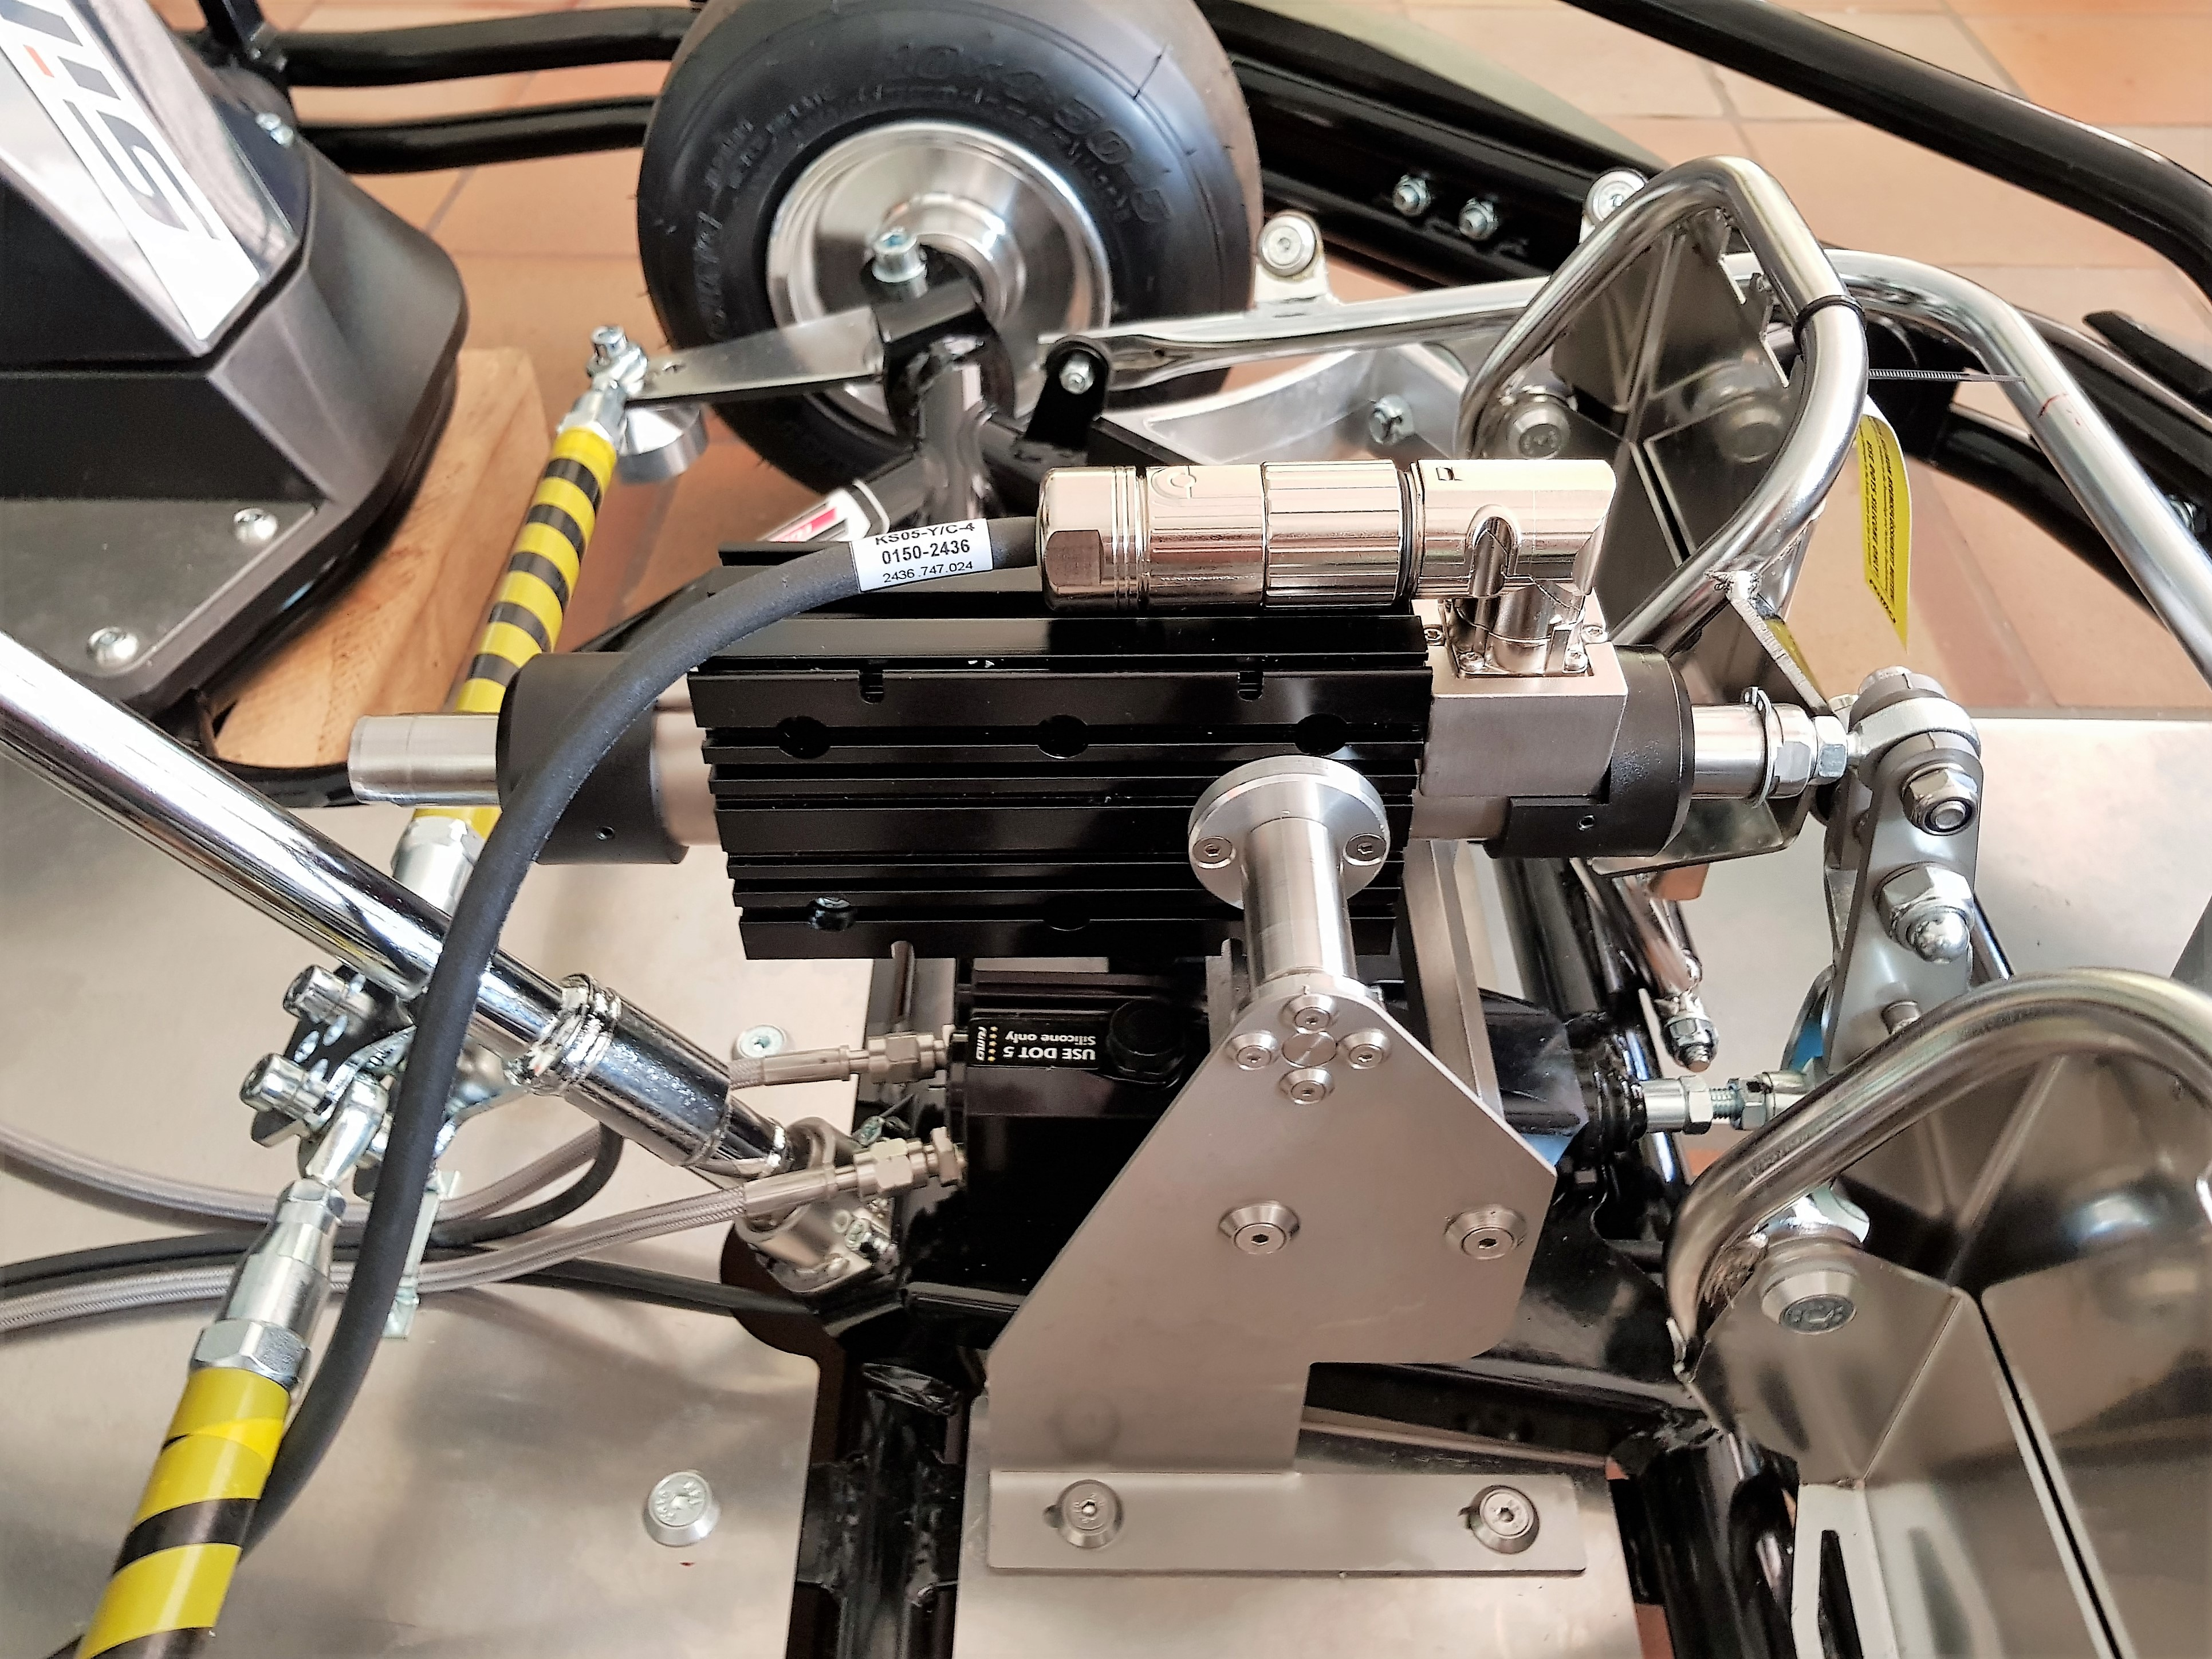
\includegraphics[width=0.7\linewidth]{pictures_figures/Used/Picture_brake}
	\caption{}
	\label{fig:picturebrake}
\end{figure}


\subsection{Throttle}

To control the throttle, we had to access the ACD 4805 motor controller of each electric drive. After a simple start up sequence, we were able to control the velocity of each wheel via CANOpen. For throttling, no actuators had to implemented. The crucial work that went into throttle-by-wire part was mainly communication and will therefore be discussed in the following chapter.

\newpage

\subsection{Steering}

As already mentioned in chapter one, we used a compact power steering unit, with a rated torque of around 3 Nm. In order to install the unit, the kart's steering column was cut up, as was the power steering's drive shaft. The column and the drive shaft were then joined together by using press-fit joints. To counter the motor's torque, we fixed it to the steering wheel's metal holder and reinforced it with an additional steel linkage.

\begin{figure}[h]
	\centering
	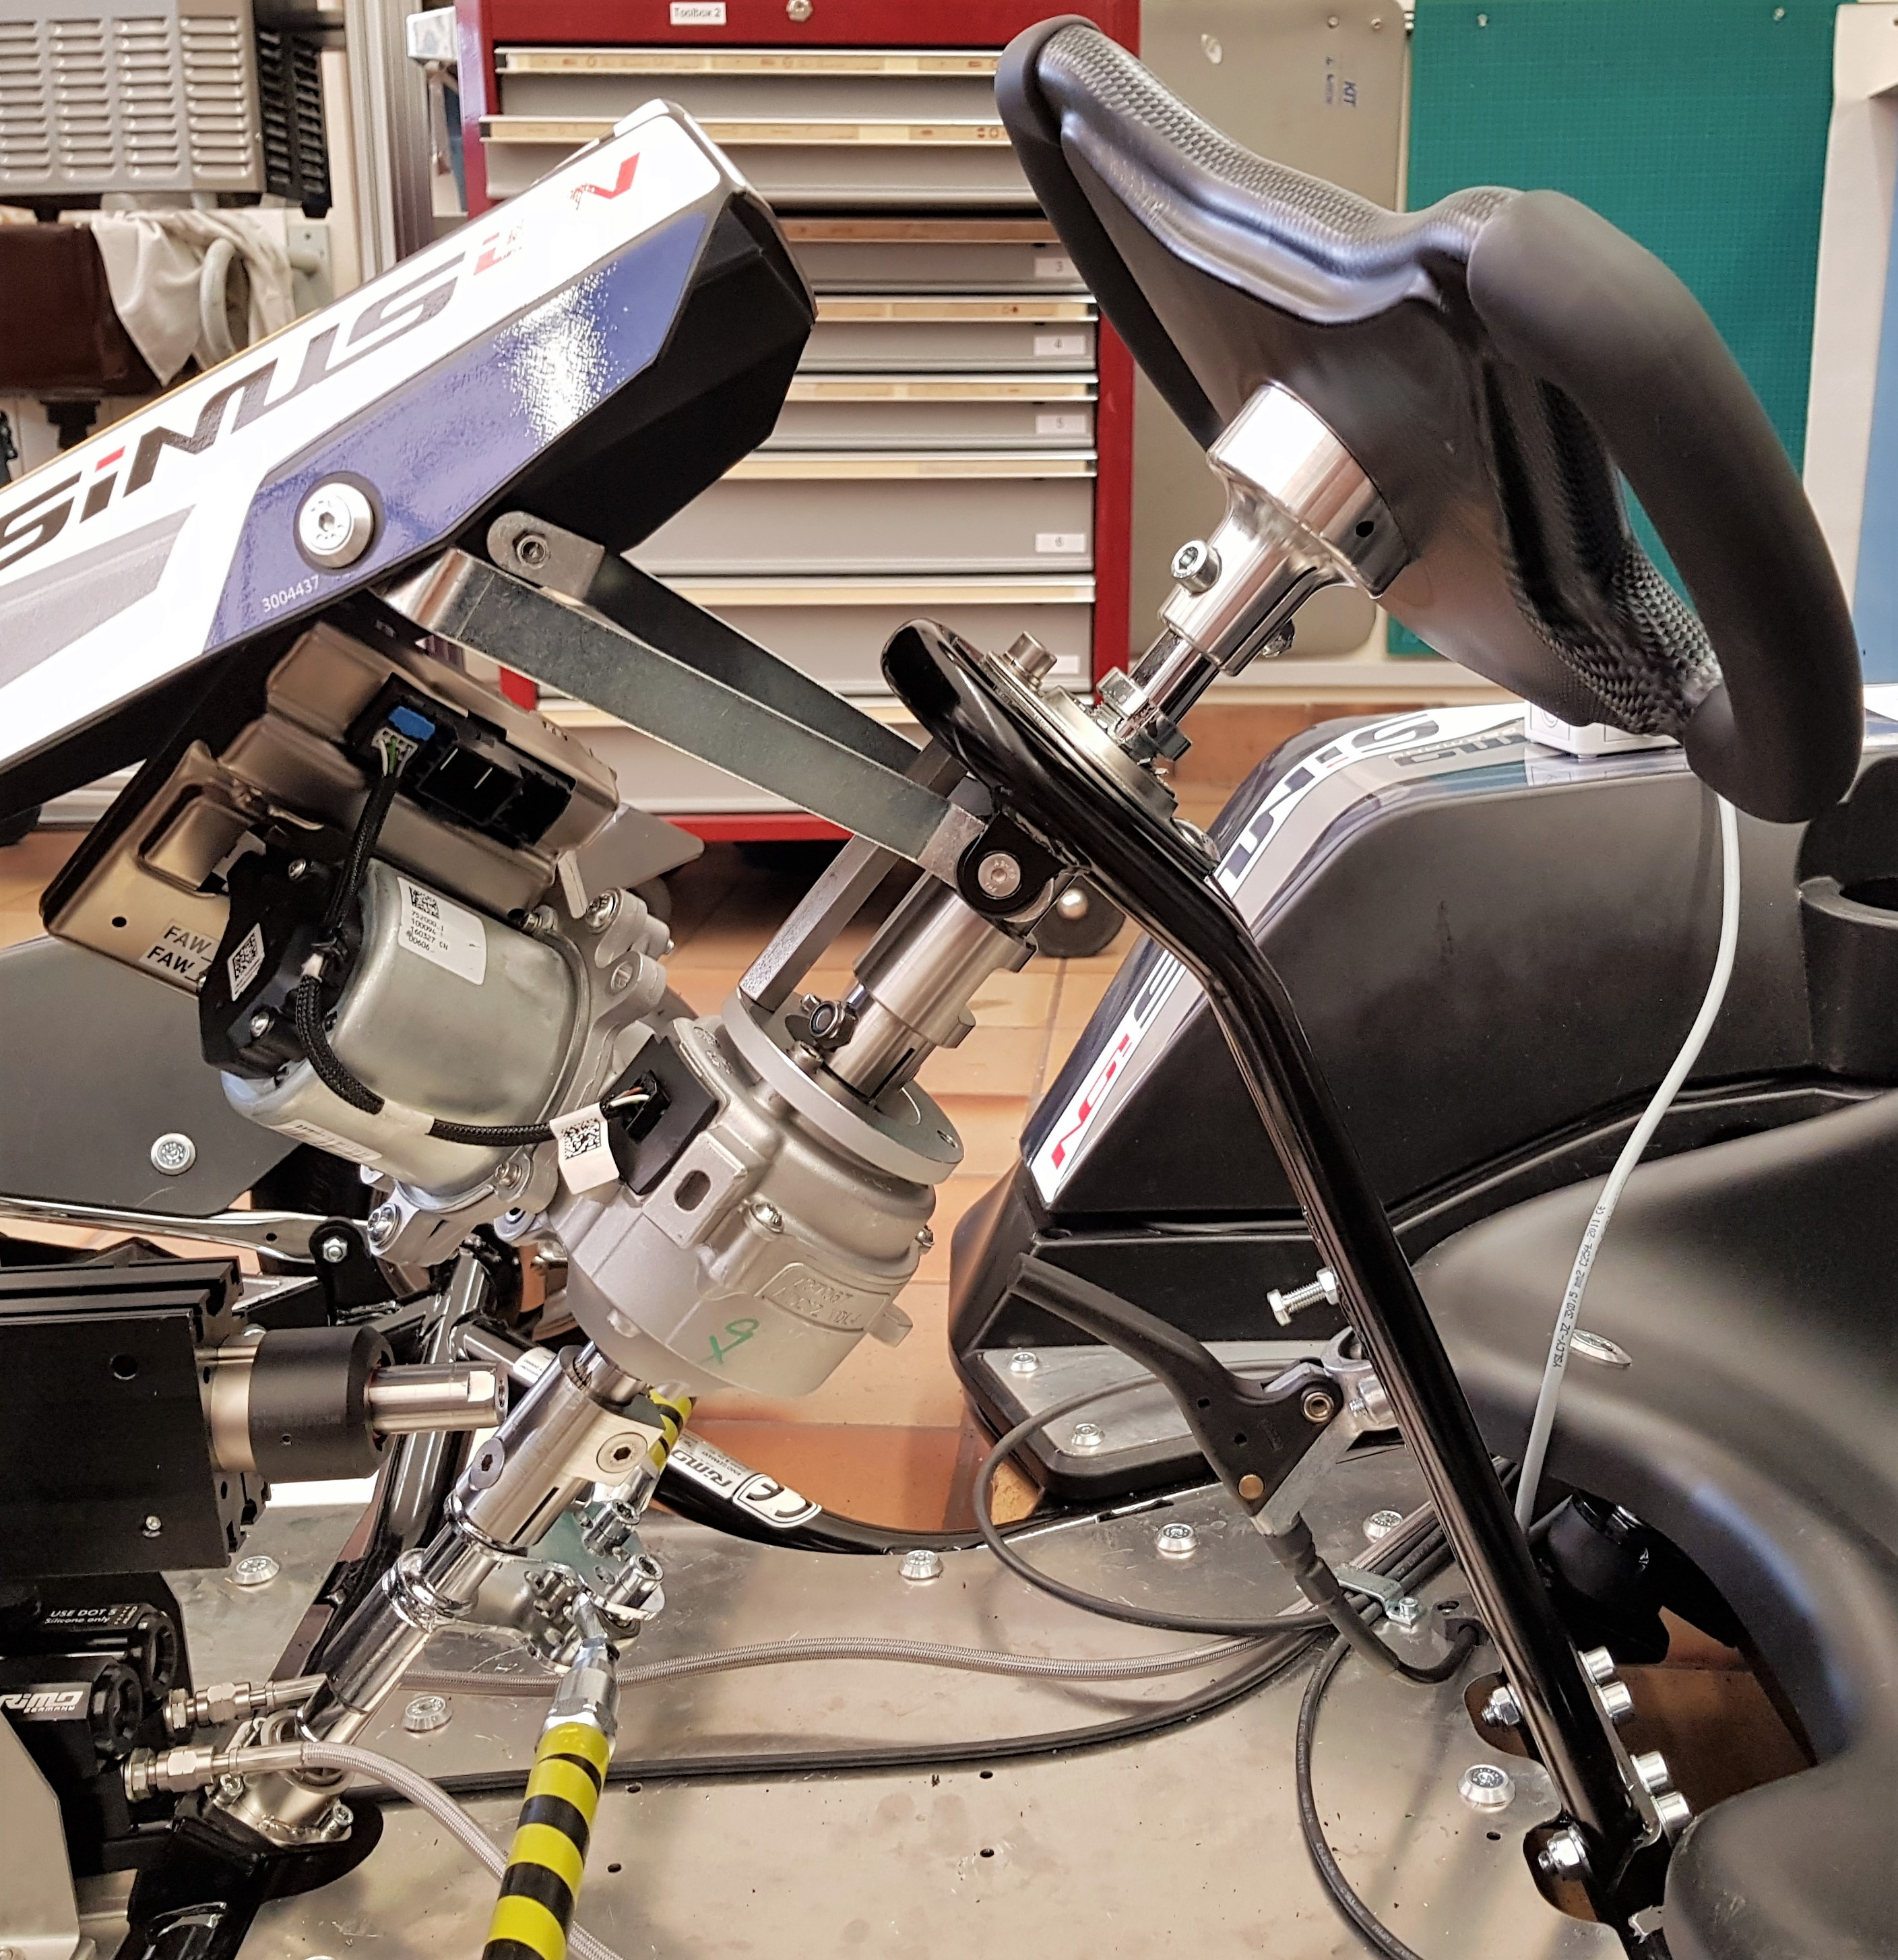
\includegraphics[width=0.7\linewidth]{pictures_figures/Used/picture_powersteering}
	\caption{}
	\label{fig:picturepowersteering}
\end{figure}

\section{Implementation Communication}

\subsection{ACD}
%explain what commands we used, object dictionary and relevant commands/messages.



%write about RPDO1 RPDO2 conflict, our assumptions what if couldve been, namely phyiscal connection, sync messages, overload, messages overlapping etc. solved by disabling rpdo2

In order to communicate with the ACD, the CAN Node-Id of each ACD had to be determined. One of Rimo's pdf files, namely "Setting up ACD Controller \& Connection Diagram", serves exactly this purpose. 
%refer to appendix witht file.
To find the respective node-id's, we had to check if either pin 12 (DI5) or pin 20 (DI6) was connected to any other pins on the ACD 4805 K1 connector. In our case, pin 12 of the right ACD was connected to pin 1, making it node 6. Pin 12 of the left ACD was not connected and therefore making it node 5. Afterwards our findings were confirmed when we connected the go-kart to our CAN bus. With the help of a CAN-USB adapter, we were able to receive and send messages, and after a while controlling the kart.
Because the go-kart does not communicate via CAN by default but only for service and remote control purposes, we had to put all nodes into operational mode by sending a NMT start messages to all nodes, namely node 5 and 6.
The ID of a NMT message is 0x000, to start the nodes the instruction code 0x01 had to be used. To reach all nodes simultaneously, the node adress needed to be 0x0. 

Issues with CANOpen and dSpace. 

When we tried to control the ACD via CANOpen with the Microautobox, the communication presented itself to be an issue. The wheels were not turning smoothly, but rather interrupted from time to time. We assumed that something had to be disrupting the communication.
With the help of a CAN-USB adapter, we were able to monitor the CAN bus. After checking all physical layers, we came to the conclusion that it must be a software problem. Our first approach was to change synchronisation times. This however did not have any effect, neither did changing the baud rate or adjusting the step size for Matlab's solver.
A smooth motion of the motors could be realized by sending the Receive PDO manually via the PCAN software. The problem turned out to arise from the second Receive PDO. While the first RPDO determines the target speed for the speed controller the second RPDO provides the possibility to control the motor with via torque control. By default, the use of one of the mentioned does not disable the function of the other. This leads to critical failure causing improper motion if both RPDOs are sent simultaneously. The motor tries to achieve both, target speed and target torgue ending up rapidly switching the motor current. The problem could be solved by completely removing the second RPDO from the Matlab model. We were not able to deactivate an individual PDO's transmission in real time with dSpace CANOpen solution.



Two's complement is convenient way to store integers, such that adding and subtracting with negative numbers becomes very easy. This was used on the ACD 4805, where certain values, such as the rotational speed of the wheels, can be negative. 
The basic principles of two's complement are the following.

- Zero is represented by all 0's. 
e.g. 0 0 0 0 = 0

- The maximum positive integer is $ 2^{number of bits-1}-1 $.
So for 4 bits, the biggest integer is therefore 0 1 1 1 = 7, and not 1 1 1 1 = 15 as in the standard notation.

- if the integer is negative, 1's and 0's switch roles, starting from all one's, e.g. 1 1 1 1 = -1. This increases the range for negative numbers by one.

So for 4 bits it looks as follows.

\begin{tabular}{llll}
	0 0 0 0 = 0 & 0 1 0 0 = 4 & 1 1 1 1 = -1 & 1 0 1 1 = -5\\
	0 0 0 1 = 1 & 0 1 0 1 = 5 & 1 1 1 0 = -2 & 1 0 1 0 = -6\\
	0 0 1 0 = 2 & 0 1 1 0 = 6 & 1 1 0 1 = -3 & 1 0 0 1 = -7\\
	0 0 1 1 = 3 & 0 1 1 1 = 7 & 1 1 0 0 = -4 & 1 0 0 0 = -8
\end{tabular}

So an easy way to find the negative integer of a positive integer is to convert the desired decimal number to binary, inverting all 0's and 1's and then adding 1. A more hands on approach is to again convert to binary, starting from the right to find the first 1 and inverting all bits to the left of it.

So in order to have a rotational speed of -500 revolutions per minute, the following steps have to be taken for a signed 16 bit integer.

500 = 0 0 0 0 \: 0 0 0 1 \: 1 1 1 1 \: 0 1 0 0

Now invert all bits.

1 1 1 1 \: 1 1 1 0 \: 0 0 0 0 \: 1 0 1 1

And add 1

1 1 1 1 \: 1 1 1 0 \: 0 0 0 0 \: 1 1 0 0 = -500

The second method would result in the following steps.

Starting from the right, find first 1.

500 = 0 0 0 0 \: 0 0 0 1 \: 1 1 1 1 \: 0 \textbf{1} 0 0

Invert all consecutive bits to the left of it.

1 1 1 1 \: 1 1 1 0 \: 0 0 0 0 \: 1 \textbf{1} 0 0 = -500

If a signed integer is postive or negative is easy to spot, as it's most significant bit determines if the number is negative or positive. 1 = negative, 0 = positive.

\subsection{LinMot}
important settings

For some reason, TPDO3 and TPDO4 would not transmit their data when a sync message was sent. This was tried to solve by setting the intern event timer to around 10 ms and changing the transmission type to 254. However, after a while it would stop transmitting out of a unknown reason. As time was scarce, we simply remapped the PDOs, such that the needed data would be transmitted via TPDO2. 

%talk about failsafe for brake

Another issues presented itself while working on the brake. Previously we used a motion command called VAI go to position 16bit, which takes velocity, acceleration/deceleration and position as input and creates a curve for the linear motor, which results in the motion. However, a new command will only be executed if the last four bits of the motion command header, called command count, has changed. In the easiest way, bit 0 can be toggled. 
To avoid this, a different setting could be utilized, called PV Stream. This uses a constant stream of position and velocity inputs during a fixed streaming period, interpolates and executes the command. While this seemed very intriguing, it's implementation was not possible. For some reason an error arose, stating that our streaming was too slow. Even after checking the period time with PCAN and checking all settings, the issue could not be resolved.
After that, we went back to the prior way of setting the position.

To counteract the need for change in the command count in order for a change in motion we introduced a pulse generator into the Matlab model.
The pulse generators output is an alternating signal either being zero or one. With the signal from the pulse generator added to the command header, the command count changes every halve period of the pulse generator. With a sufficiently low pulse generator period a function similar to the PV stream could be implemented.
%%really
%clock not working as it triggers resets all the time

\subsection{Power steering}

As of now, the needed simulink blocks for the power steering have not yet arrived. Communication is therefore not yet possible with the power steering unit and will not covered in this section.




% !TeX spellcheck = en_GB
% !TeX encoding = UTF-8
% !TeX root = ../report.tex

\chapter{Results and Discussion}
\label{chp:Results}
\input{chapters/Conclusion}
% !TeX spellcheck = en_US
% !TeX encoding = UTF-8
% !TeX root = ../report.tex

\chapter{Appendix}
\label{chp:Appendix}

The following code is the definition of the bibliography entry of the document class IDSCreport~\cite{IDSCreportClass}.

\lstinputlisting[style=plaincode,xleftmargin=1em]{bibliography.bib}
\appendix
\end{document}
